\documentclass[twocolumns]{IEEEtran}
\usepackage{algorithm}
\usepackage{algpseudocode}
\usepackage{graphicx}
\usepackage{caption}
\usepackage{url}
\captionsetup{justification=centering}


\algnewcommand\algorithmicforeach{\textbf{for each}}
\algdef{S}[FOR]{ForEach}[1]{\algorithmicforeach\ #1\ \algorithmicdo}

\author{Erdal Sidal Dogan, Alp Gokcek \\ MEF University \\ \today}
\title{Dijkstra's Shortest Path Algorithm Implementation \& Visualization}


\begin{document}
	\maketitle
	\begin{abstract}
		Dijkstra's Shortest Path Algorithm \cite{dijkstra} is an algorithm which finds the shortest path between two nodes in a graph. It is widely used and adopted for many different applications, such as computer networks, road maps, social platforms etc. In this project we implemented algorithm in Python Language and visualized the shortest path.
	\end{abstract}
	\begin{IEEEkeywords}
		Graph, Node, Vertex, Edge
	\end{IEEEkeywords}
	\section{Introduction}
	\textit{Dijkstra's Algorithm} calculates the shortest path from one desired node of the graph to every other nodes. There are varios implementations of the algorithm, main difference between them is how they store the verticies of the graph, denoted with $Q$. They can be stored in regular arrays, linked lists, adjacency lists or tree structures.\cite{524471} Running time of the algorithm can be represented with number of edges $|E|$ and number of verticies $|V|$ using big-o notation. Running time mainly depends on these structures, storing $Q$ in arrays it is $\mathcal{O}(|V|^2)$. In this project we utilized the \textit{priority queue} structure while implementing. It is more efficient way to implement comparing to arrays and adjacency lists etc. The \textit{priority queue} implementation requires $\mathcal{O}((|E| + |V|) \log{|V|})$ time in the worst case. 
	\begin{algorithm}
		\caption{Using a priority queue \cite{wiki} \hfill Cost}
		\begin{algorithmic}[1]
			\Function {Dijkstra} {\textit{Graph, source}}
				\ForEach {vertex \textbf{v} in \textit{Graph}}	\hfill v + 1
					\State $dist[v] \leftarrow$ INFINITY	\hfill v
					\State $prev[v] \leftarrow$ UNDEFINED	\hfill v
					\State add $v$ to $Q$	\hfill v                      
				\EndFor
				\State $dist[source] \leftarrow$ 0	\hfill 1
	
				\While {$Q$ is not empty}	\hfill v + 1
					\State $u \leftarrow$ vertex in $Q$ with min $dist[u]$	\hfill v
					\State remove $u$ from $Q$	\hfill v
					\ForEach {neighbor $v$ of $u$}	\hfill $\sum_{i=0}^{v}(v-i+2)$
						\State $alt \leftarrow dist[u] + length(u, v)$ $\sum_{i=0}^{v}(v-i+1)$
						\If{alt $<$ dist[v]}	\hfill $\sum_{i=0}^{v}(v-i+2)$
							\State $dist[v] \leftarrow alt$	\hfill $\sum_{i=0}^{v}(v-i+2)$
							\State $prev[v] \leftarrow u$	\hfill $\sum_{i=0}^{v}(v-i+2)$
						\EndIf
					\EndFor
				\EndWhile \\
				\Return dist[], prev[]
			\EndFunction
		\end{algorithmic}
	\end{algorithm}

	\section{The Program}

	The program consists a simple and intuitive Graphical User Interface. On the top there are text fields where the user can type de number of nodes, start node and the destination node respectively. Below, there is the path from source to destination and time it took to travel between these nodes. Rest of the application window displays the nodes and emphasizes the shortest path between two given nodes in red color edges.

	\begin{figure}[h]
		\centering
		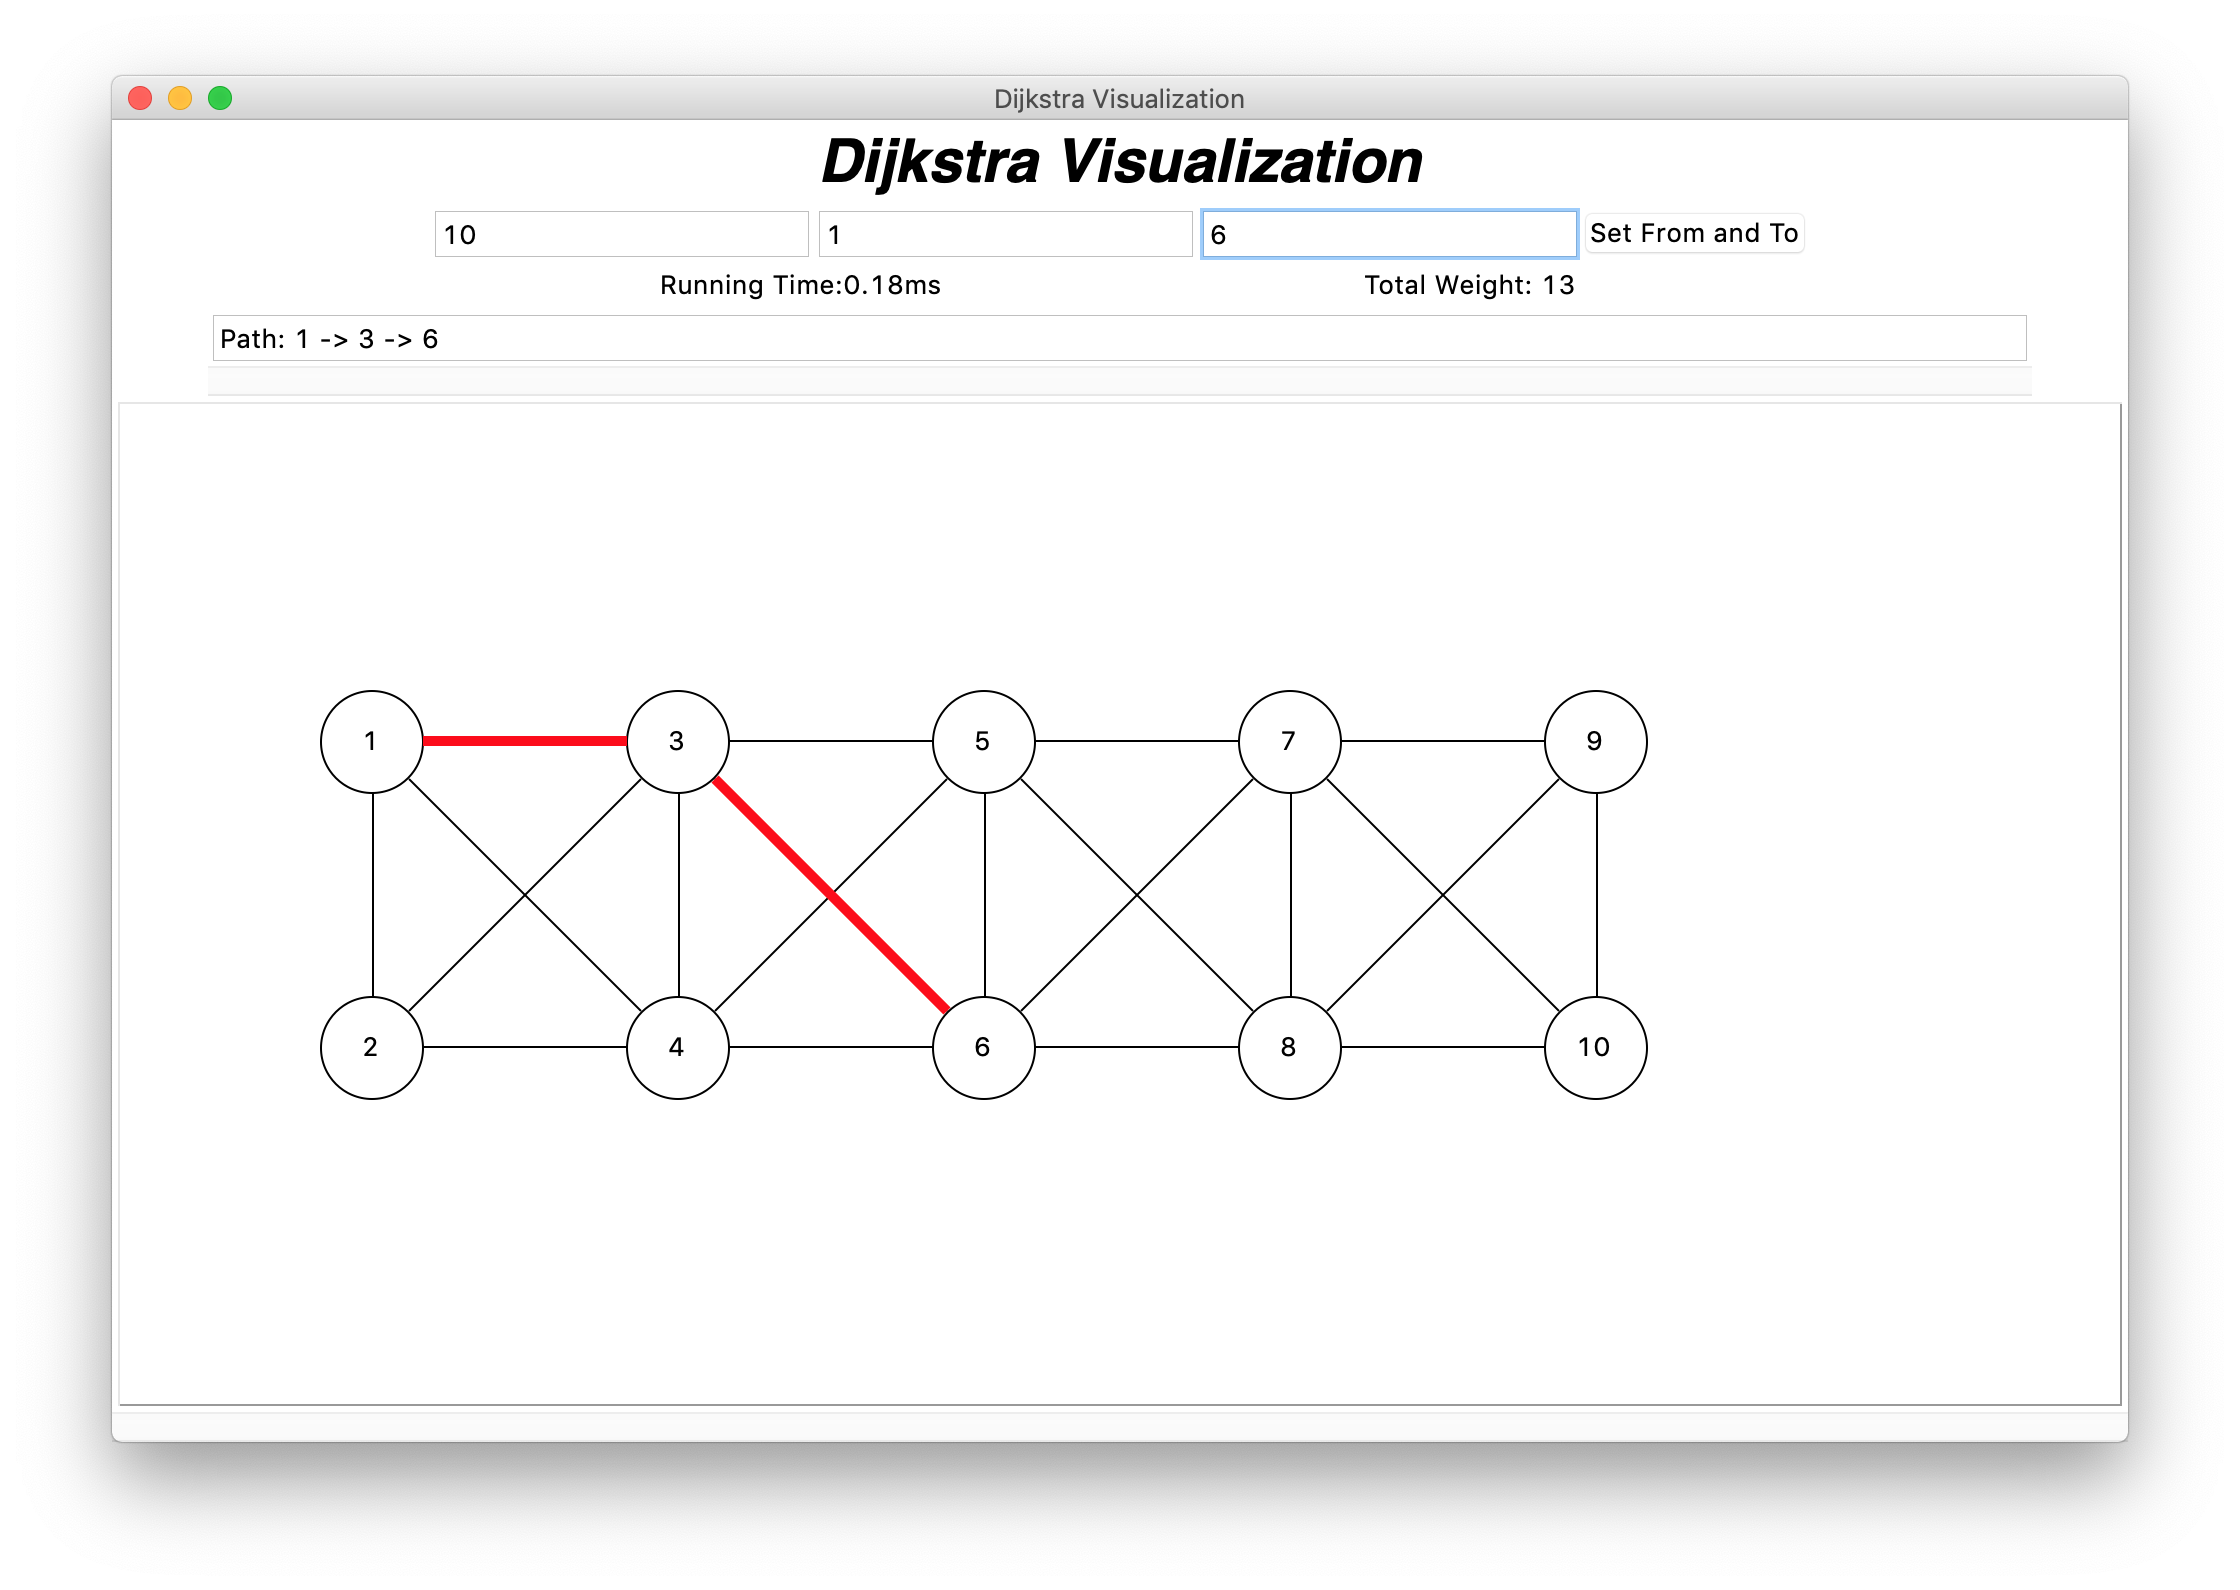
\includegraphics[scale=.2]{main_window.png}
	\end{figure}
	\captionof{figure}{Main Window of the program for values selected as; N=10, S=1, D=6} 
	
	\section{Time Measurements}
	
	After the implementation, we measured the time it takes to calculate shortest path from 1 to $N$ in a graph with $N$ number of nodes. We observed a correlation between theory and the practice.
	Theoritical results are calculated by the $\mathcal{O}((|E| + |V|) \log{|V|})$ which stated in \textit{Introduction} section previously. Time it takes to run the program depends on the computer it ran on. During our demonstration we used the same machine with same configuration in order to get most accurate results. For different machines the expectation is to get ratios that are closer to ratio of our results. Results can be seen in detail from the figure below; \\
	
	\begin{figure}
		\centering
		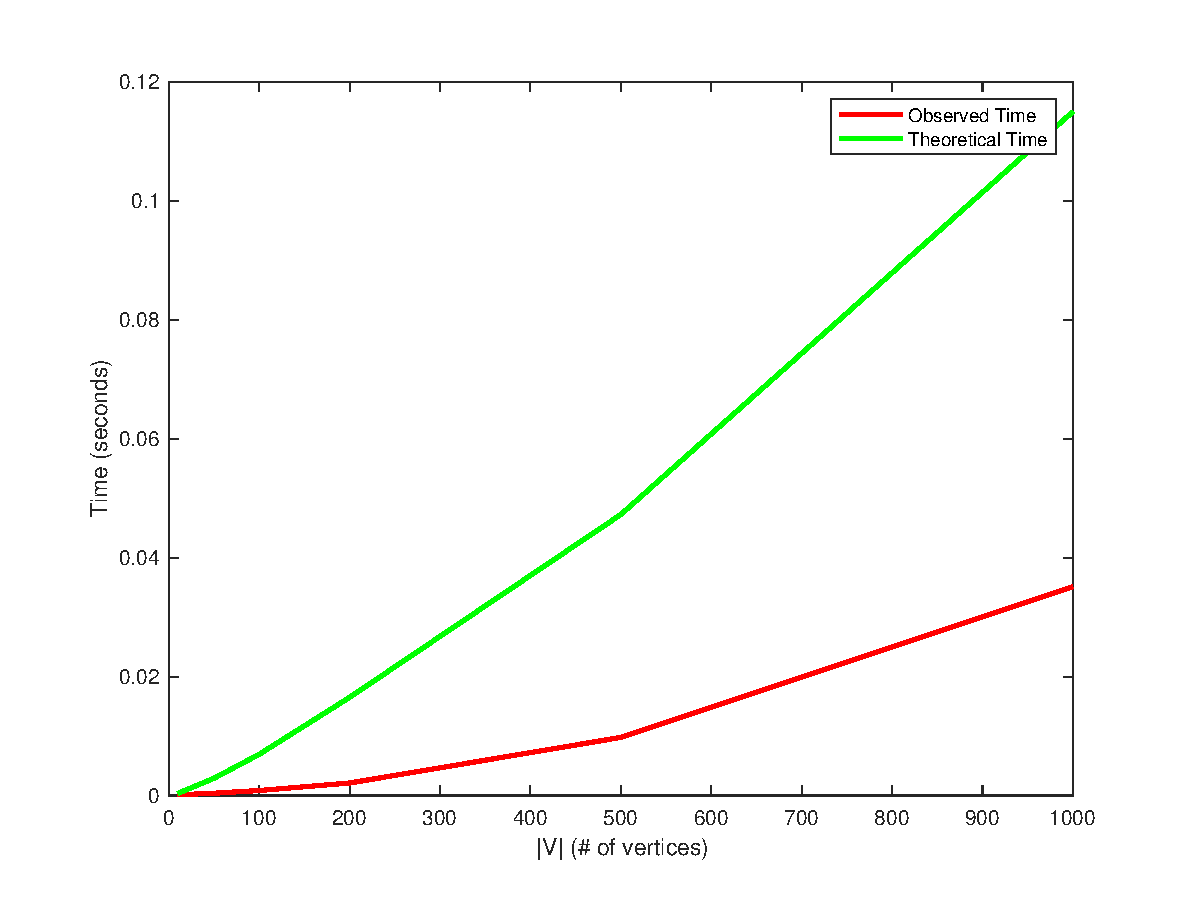
\includegraphics[scale=.4]{matlab/time_2.eps}
		\caption{$|V|$ vs. time (in seconds)}
	\end{figure}

	Note that theoretical time (showed in green line) doesn't correspond to any value of time, it is put there to emphasize the overall similarities such as curvature and trajectory etc. between actual results and calculated results.
	

	\section{Conclusion \& Discussion}
	In this project we implemented \textit{Dijkstra's Algorithm} using Python. We developed an GUI in order to visualize the graph and the shortest path. After the implementation, we compared our results with the theoritical results. This project helped us to develop a deeper insight about the graphs and the shortest path algorithms.

	\bibliographystyle{IEEEtran}
	\bibliography{references}

\end{document}